\documentclass{standalone}
\usepackage{tikz}
\begin{document}
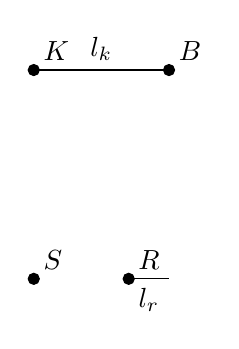
\begin{tikzpicture}[scale=1.0]
  \filldraw (0.0, 0.0) circle (2pt) node[above right] {$K$};
  \filldraw (1.7177, 0.0) circle (2pt) node[above right] {$B$};
  \filldraw (0.0, -2.6515) circle (2pt) node[above right] {$S$};
  \filldraw (1.2056, -2.6515) circle (2pt) node[above right] {$R$};
  \draw (0.0, 0.0) -- (1.7177, 0.0) node[midway, above] {$l_k$};
  \draw (1.2056, -2.6515) -- (1.7177, -2.6515) node[midway, below] {$l_r$};
\end{tikzpicture}
\end{document}